\documentclass[a4paper]{article}%formato de plantilla%
\usepackage[utf8]{inputenc}
\usepackage[spanish]{babel}
\usepackage[margin=2cm, top=2cm, includefoot]{geometry}
\usepackage{graphicx} %para la insercion de imagenes 
\usepackage[table,xcdraw]{xcolor} % Para la deteccion de colores
\usepackage[most]{tcolorbox} % Para la insercion de cuadores en la portada
\usepackage{fancyhdr} %Definir el estilo de la pagina 
\usepackage[hidelinks]{hyperref} % Gestion de hipervinculos
\usepackage{parskip} %Arreglo d la tabulacion en el documento
\usepackage[figurename=Figura]{caption} % Cambiar el nombre del caption de las fotos
\usepackage{smartdiagram} % Para la insercion de diagramas 


%Declaracion de colores 
\definecolor{greenPortada}{HTML}{69A84F}

%Declaracion de variables%
\newcommand{\logoPortada}{thm.png}
\newcommand{\machineName}{Blue} %nombre de la maquina
\newcommand{\logoMachine}{machine.png} % logo de la maquina
\newcommand{\startDate}{29 de Octubre del 2020}

% Adicionales 
\addto\captionsspanish{\renewcommand{\contentsname}{Indice}} % Cambio del formato del Indice
\setlength{\headheight}{40.2pt}
\pagestyle{fancy}
\fancyhf{}
\lhead{\includegraphics[width=2.5cm]{\logoPortada}}\rhead{\includegraphics[height=1.5cm]{\logoMachine}}
\renewcommand{\headrulewidth}{3pt}
\renewcommand{\headrule}{\hbox to\headwidth{\color{greenPortada}\leaders\hrule height \headrulewidth\hfill}}


%Comienzo del documento 
\begin{document}
	\cfoot{\thepage}
	%Creacion de portada 
	\begin{titlepage}
	\centering
	\includegraphics[width=0.5\textwidth]{\logoPortada}\par\vspace{1cm}
	{\scshape\LARGE \textbf{Informe Tecnico}\par }
	\vspace{0.2cm}
	{\Huge\bfseries\textcolor{greenPortada}{Room \machineName}\par}
	\vfill\vfill
	\includegraphics[width=\textwidth,height=8cm,keepaspectratio]{\logoMachine}\par\vspace{1cm}
	\vfill
	\begin{tcolorbox}[colback=red!5!white,colframe=red!75!black]
		\centering
		Este documento es confidencial y contiene informacion sensible.\\No deberia
		ser impreso o compartido con terceras entidades.
	\end{tcolorbox}	
	\vfill
	{\large \startDate\par}
	\vfill
	\end{titlepage}
	%--------------------------------------------- 
	%Comienzo del TOC
	\clearpage
	\tableofcontents
	\clearpage
	%--------------------------------------------
	\section{Antecendentes}
	El presente documento recoge los resultados obtenidos durante la fase de auditoria
	realizada a la maquina {\textbf\machineName} de la plataforma 
	\href{https://tryhackme.com}{\textbf{Tryhackme}}. 
	\vspace{0.2cm}

	\section{Analisis de vulnerabilidades}
	\subsection{Reconocimiento inicial}

	\vspace{0.2cm}
	Se comenzo realizando un analisis inicial sobre el sistema, verificando que el sistema
	objetivo se encontrara accesible desde el segmento de red en el que se opera:

	\begin{verbatim}
		ping -c5 ip
	\end{verbatim}

	% foto del ping
	\begin{figure}[h]
	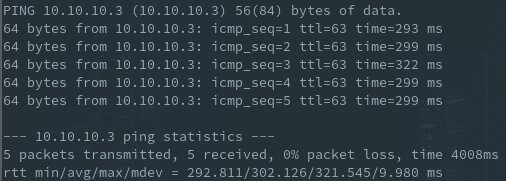
\includegraphics[width=0.7\textwidth]{ping.png}
	\end{figure}

	\vspace{0.2cm}

	\subsection{Reconocimento por Servicios}
	
	Una vez localizado, se realizo un escaneo a traves de la herramienta \textbf{nmap}
	para la deteccion de puertos abiertos.

	\begin{verbatim}
	nmap -p- -n 
	\end{verbatim}

	% foto del nmap con servicios y scripts basicos
	\begin{figure}[h]
	\includegraphics[width=0.7\textwidth]{ports.png}
	\end{figure}

	Una vez identificado los puertos utilizamos los 
	scripts de nmap que nos permiten ver las 
	posibles vulnerabilidades del sistemas.

	\includegraphics[width=0.7\textwidth]{nmap_script.png}


	\section{Explotacion}
	Para esta explotacion usamos la herramienta Autoblue

	\begin{verbatim}
	https://github.com/3ndG4me/AutoBlue-MS17-010
	\end{verbatim}

	\subsection{Crear shellcode}

	Con estos comandos se crean dos shellcodes(para la 
	arquitectura x86 y x64) para el script a partir de 
	sus herramientas de reconocimiento va a identificar 
	una y con el puerto que le indiques para 
	cada arquitectura se generar conexion.
	
	\includegraphics[width=0.7\textwidth]{shellcode.png}

	\subsection{Obteniendo acceso}

	antes de correr el exploit ponemos nuestros puertos 
	indicados a la escucha y esperamos.

	\newpage
	
	\includegraphics[width=0.7\textwidth]{explotacion.png}

	\includegraphics[width=0.7\textwidth]{netcat.png}

	y como se puede ver en esta imagen la vulnerabilidad
	EternalBlue nos autentica como root.
	
	\includegraphics[width=0.7\textwidth]{privesc.png}
		
\end{document}
